\documentclass[journal,12pt,twocolumn]{IEEEtran}
\usepackage{setspace}
\usepackage{gensymb}
\usepackage{caption}
%\usepackage{multirow}
%\usepackage{multicolumn}
%\usepackage{subcaption}
%\doublespacing
\singlespacing
\usepackage{csvsimple}
\usepackage{amssymb}
\usepackage{amsmath}
\usepackage{multicol}
%\usepackage{enumerate}
\usepackage{amssymb}
%\usepackage{graphicx}
\usepackage{newfloat}
%\usepackage{syntax}
\usepackage{listings}
\usepackage{color}
\usepackage{tikz}
\usepackage{graphicx}
\usetikzlibrary{shapes,arrows}

%\usepackage{graphicx}
%\usepackage{amssymb}
%\usepackage{relsize}
%\usepackage[cmex10]{amsmath}
%\usepackage{mathtools}
%\usepackage{amsthm}
%\interdisplaylinepenalty=2500
%\savesymbol{iint}
%\usepackage{txfonts}
%\restoresymbol{TXF}{iint}
%\usepackage{wasysym}
\usepackage{amsthm}
\usepackage{mathrsfs}
\usepackage{txfonts}
\usepackage{stfloats}
\usepackage{cite}
\usepackage{cases}
\usepackage{mathtools}
\usepackage{caption}
\usepackage{enumerate}	
\usepackage{enumitem}
\usepackage{amsmath}
%\usepackage{xtab}
\usepackage{longtable}
\usepackage{multirow}
%\usepackage{algorithm}
%\usepackage{algpseudocode}
\usepackage{enumitem}
\usepackage{mathtools}
\usepackage{hyperref}
%\usepackage[framemethod=tikz]{mdframed}
\usepackage{listings}
    %\usepackage[latin1]{inputenc}                                 %%
    \usepackage{color}                                            %%
    \usepackage{array}                                            %%
    \usepackage{longtable}                                        %%
    \usepackage{calc}                                             %%
    \usepackage{multirow}                                         %%
    \usepackage{hhline}                                           %%
    \usepackage{ifthen}                                           %%
  %optionally (for landscape tables embedded in another document): %%
    \usepackage{lscape}     


\usepackage{url}
\def\UrlBreaks{\do\/\do-}


%\usepackage{stmaryrd}


%\usepackage{wasysym}
%\newcounter{MYtempeqncnt}
\DeclareMathOperator*{\Res}{Res}
%\renewcommand{\baselinestretch}{2}
\renewcommand\thesection{\arabic{section}}
\renewcommand\thesubsection{\thesection.\arabic{subsection}}
\renewcommand\thesubsubsection{\thesubsection.\arabic{subsubsection}}

\renewcommand\thesectiondis{\arabic{section}}
\renewcommand\thesubsectiondis{\thesectiondis.\arabic{subsection}}
\renewcommand\thesubsubsectiondis{\thesubsectiondis.\arabic{subsubsection}}

% correct bad hyphenation here
\hyphenation{op-tical net-works semi-conduc-tor}

%\lstset{
%language=C,
%frame=single, 
%breaklines=true
%}

%\lstset{
	%%basicstyle=\small\ttfamily\bfseries,
	%%numberstyle=\small\ttfamily,
	%language=Octave,
	%backgroundcolor=\color{white},
	%%frame=single,
	%%keywordstyle=\bfseries,
	%%breaklines=true,
	%%showstringspaces=false,
	%%xleftmargin=-10mm,
	%%aboveskip=-1mm,
	%%belowskip=0mm
%}

%\surroundwithmdframed[width=\columnwidth]{lstlisting}
\def\inputGnumericTable{}                                 %%
\lstset{
%language=C,
frame=single, 
breaklines=true,
columns=fullflexible
}

\begin{document}
%
\tikzstyle{block} = [rectangle, draw,
    text width=3em, text centered, minimum height=3em]
\tikzstyle{sum} = [draw, circle, node distance=3cm]
\tikzstyle{input} = [coordinate]
\tikzstyle{output} = [coordinate]
\tikzstyle{pinstyle} = [pin edge={to-,thin,black}]

\theoremstyle{definition}
\newtheorem{theorem}{Theorem}[section]
\newtheorem{problem}{Problem}
\newtheorem{proposition}{Proposition}[section]
\newtheorem{lemma}{Lemma}[section]
\newtheorem{corollary}[theorem]{Corollary}
\newtheorem{example}{Example}[section]
\newtheorem{definition}{Definition}[section]
%\newtheorem{algorithm}{Algorithm}[section]
%\newtheorem{cor}{Corollary}
\newcommand{\BEQA}{\begin{eqnarray}}
\newcommand{\EEQA}{\end{eqnarray}}
\newcommand{\define}{\stackrel{\triangle}{=}}

\bibliographystyle{IEEEtran}
%\bibliographystyle{ieeetr}

\providecommand{\nCr}[2]{\,^{#1}C_{#2}} % nCr
\providecommand{\nPr}[2]{\,^{#1}P_{#2}} % nPr
\providecommand{\mbf}{\mathbf}
\providecommand{\pr}[1]{\ensuremath{\Pr\left(#1\right)}}
\providecommand{\qfunc}[1]{\ensuremath{Q\left(#1\right)}}
\providecommand{\sbrak}[1]{\ensuremath{{}\left[#1\right]}}
\providecommand{\lsbrak}[1]{\ensuremath{{}\left[#1\right.}}
\providecommand{\rsbrak}[1]{\ensuremath{{}\left.#1\right]}}
\providecommand{\brak}[1]{\ensuremath{\left(#1\right)}}
\providecommand{\lbrak}[1]{\ensuremath{\left(#1\right.}}
\providecommand{\rbrak}[1]{\ensuremath{\left.#1\right)}}
\providecommand{\cbrak}[1]{\ensuremath{\left\{#1\right\}}}
\providecommand{\lcbrak}[1]{\ensuremath{\left\{#1\right.}}
\providecommand{\rcbrak}[1]{\ensuremath{\left.#1\right\}}}
\theoremstyle{remark}
\newtheorem{rem}{Remark}
\newcommand{\sgn}{\mathop{\mathrm{sgn}}}
\providecommand{\abs}[1]{\left\vert#1\right\vert}
\providecommand{\res}[1]{\Res\displaylimits_{#1}} 
\providecommand{\norm}[1]{\left\Vert#1\right\Vert}
\providecommand{\mtx}[1]{\mathbf{#1}}
\providecommand{\mean}[1]{E\left[ #1 \right]}
\providecommand{\fourier}{\overset{\mathcal{F}}{ \rightleftharpoons}}
\providecommand{\gauss}[2]{\mathcal{N}\ensuremath{\left(#1,#2\right)}}
%\providecommand{\hilbert}{\overset{\mathcal{H}}{ \rightleftharpoons}}
\providecommand{\system}{\overset{\mathcal{H}}{ \longleftrightarrow}}
	%\newcommand{\solution}[2]{\textbf{Solution:}{#1}}
\newcommand{\solution}{\noindent \textbf{Solution: }}
\newcommand{\myvec}[1]{\ensuremath{\begin{pmatrix}#1\end{pmatrix}}}
\providecommand{\dec}[2]{\ensuremath{\overset{#1}{\underset{#2}{\gtrless}}}}
\DeclarePairedDelimiter{\ceil}{\lceil}{\rceil}
%\numberwithin{equation}{section}
%\numberwithin{problem}{subsection}
%\numberwithin{definition}{subsection}
\makeatletter
\@addtoreset{figure}{section}
\makeatother

\let\StandardTheFigure\thefigure
%\renewcommand{\thefigure}{\theproblem.\arabic{figure}}
\renewcommand{\thefigure}{\thesection}


%\numberwithin{figure}{subsection}

%\numberwithin{equation}{subsection}
%\numberwithin{equation}{section}
%\numberwithin{equation}{problem}
%\numberwithin{problem}{subsection}
\numberwithin{problem}{section}
%%\numberwithin{definition}{subsection}
%\makeatletter
%\@addtoreset{figure}{problem}
%\makeatother
\makeatletter
\@addtoreset{table}{section}
\makeatother

\let\StandardTheFigure\thefigure
\let\StandardTheTable\thetable
\let\vec\mathbf
\numberwithin{equation}{section}

\vspace{3cm}


\title{%Convex Optimization in Python
	Random Numbers
}
%\title{
%	\logo{Matrix Analysis through Octave}{\begin{center}\includegraphics[scale=.24]{tlc}\end{center}}{}{HAMDSP}
%}

% paper title
% can use linebreaks \\ within to get better formatting as desired
%\title{Matrix Analysis through Octave}
%
%
% author names and IEEE memberships
% note positions of commas and nonbreaking spaces ( ~ ) LaTeX will not break
% a structure at a ~ so this keeps an author's name from being broken across
% two lines.
% use \thanks{} to gain access to the first footnote area
% a separate \thanks must be used for each paragraph as LaTeX2e's \thanks
% was not built to handle multiple paragraphs
%

\author{JARPULA BHANU PRASAD - AI21BTECH11015}
\maketitle

\tableofcontents

\bigskip

\renewcommand{\thefigure}{\theenumi}
\renewcommand{\thetable}{\theenumi}

\begin{abstract}
This manual provides a simple introduction to the generation of random numbers
\end{abstract}
%%
\section{Uniform Random Numbers}
Let $U$ be a uniform random variable between 0 and 1.
\begin{enumerate}[label=\thesection.\arabic*
,ref=\thesection.\theenumi]
\item Generate $10^6$ samples of $U$ using a C program and save into a file called uni.dat .\\
\solution
Download the following files and execute the C program
\begin{lstlisting}
$ wget https://github.com/jarpula-Bhanu/Random-numbers/blob/main/codes/exrand.c
$ wget https://github.com/jarpula-Bhanu/Random-numbers/blob/main/codes/coeffs.h
\end{lstlisting}
Compile and execute the above C program using command
\begin{lstlisting}
$ gcc exrand.c -lm -o exrand.out
$ ./exrand.out
\end{lstlisting}

%
\item
Load the uni.dat file into python and plot the empirical CDF of $U$ using the samples in uni.dat. The CDF is defined as
\begin{align}
F_{U}(x) = \pr{U \leq x}
\end{align}

\solution  The following code plots Fig. \ref{fig:uni_cdf}
\begin{lstlisting}
$ wget https://github.com/jarpula-Bhanu/Random-numbers/blob/main/codes/cdf_plot.py
\end{lstlisting}
The above code is executed using command
\begin{lstlisting}
$ python3 cdf_plot.py
\end{lstlisting}

\begin{figure}[h]
\centering
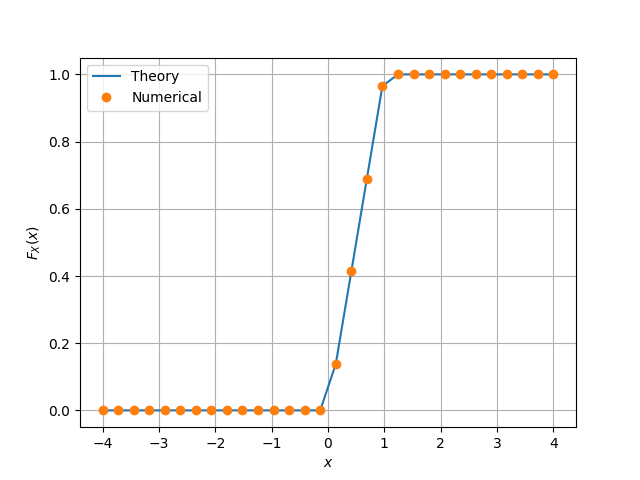
\includegraphics[width=\columnwidth]{uni_cdf.png}
\caption{The CDF of $U$}
\label{fig:uni_cdf}
\end{figure}

%
\item
Find a theoretical expression for $F_{U}(x)$.

\solution Since $U$ is a uniformly distributed in [0,1]  \\
We have three cases:
\begin{itemize}
\item $x < 0$: $P_X(x) = 0$, and hence $F_U(x) = 0$.
\item $0 \leq x < 1$: Here,
\begin{align}
    F_U(x) = \int_{0}^{x}du = x
\end{align}
\item $x \geq 1$: Put $x = 1$ in above eqn we get $F_U(x) = 1$.
\end{itemize}
Therefore,
\begin{align}
    F_U(x) = 
    \begin{cases}
        0 & x < 0 \\
        x & 0 \leq x < 1 \\
        1 & x \geq 1
    \end{cases}
\end{align}
This can be verified from Fig. \ref{fig:uni_cdf} 

\item
The mean of $U$ is defined as
%
\begin{equation}
E\sbrak{U} = \frac{1}{N}\sum_{i=1}^{N}U_i
	\label{eq:mean-form}
\end{equation}
%
and its variance as
%
\begin{equation}
\text{var}\sbrak{U} = E\sbrak{U- E\sbrak{U}}^2 
	\label{eq:var-form}
\end{equation}

Write a C program to  find the mean and variance of $U$.

\solution Download the following files and execute the C program
\begin{lstlisting}
$ wget https://github.com/jarpula-Bhanu/Random-numbers/blob/main/codes/exrand.c
$ wget https://github.com/jarpula-Bhanu/Random-numbers/blob/main/codes/coeffs.h
\end{lstlisting}
Compile and execute the above C program using command
\begin{lstlisting}
$ gcc exrand.c -lm -o exrand.out
$ ./exrand.out
\end{lstlisting}

The mean of $U$ is 0.500007\\
The varience of $U$ is 0.083301 \\

\item Verify your result theoretically given that
\end{enumerate}
%
\begin{equation}
E\sbrak{U^k} = \int_{-\infty}^{\infty}x^kdF_{U}(x)dx
\end{equation}
\solution Verifying result theoritically\\
Given that
\begin{align}
    E[U^k] &= \int_{-\infty}^{\infty} x^k dF_U(x)
\end{align}
Mean is given by
\begin{align}
    E[U] &= \int_{-\infty}^{\infty} x dF_U(x) \\
    &= \int_{-\infty}^{\infty} x dx \\
    &= \bigg[\frac{x^2}{2}\bigg]_0^1 \\
    &= \frac{1}{2}
\end{align}
Varaience is given by
\begin{align}
    E[U-E[U]]^2 &= E[U^2] - E[U]^2 \\
    E[U]^2 &= \int_{-\infty}^{\infty} x^2 dF_U(x)\\
    &= \int_{-\infty}^{\infty} x^2 dx \\
    &= \bigg[\frac{x^3}{3}\bigg]_0^1 \\
    &= \frac{1}{3} \\
    E[U-E[U]]^2 &= \frac{1}{3} - (\frac{1}{2})^2 \\
    &= \frac{1}{3} - \frac{1}{4} \\
    &= \frac{1}{12}
\end{align}

\section{Central Limit Theorem}
%
\begin{enumerate}[label=\thesection.\arabic*
,ref=\thesection.\theenumi]

%
\item
Generate $10^6$ samples of the random variable
%
\begin{equation}
X = \sum_{i=1}^{12}U_i -6
\end{equation}
%
using a C program, where $U_i, i = 1,2,\dots, 12$ are  a set of independent uniform random variables between 0 and 1
and save in a file called gau.dat

\solution
Download the following files and execute the C program
\begin{lstlisting}
$ wget https://github.com/jarpula-Bhanu/Random-numbers/blob/main/codes/exrand.c
$ wget https://github.com/jarpula-Bhanu/Random-numbers/blob/main/codes/coeffs.h
\end{lstlisting}
Compile and execute the above C program using command
\begin{lstlisting}
$ gcc exrand.c -lm -o exrand.out
$ ./exrand.out
\end{lstlisting}
%
\item
Load gau.dat in python and plot the empirical CDF of $X$ using the samples in gau.dat. What properties does a CDF have?

\solution The CDF of $X$ is plotted in Fig. \ref{fig:gauss_cdf}
\begin{figure}[h]
    \centering
    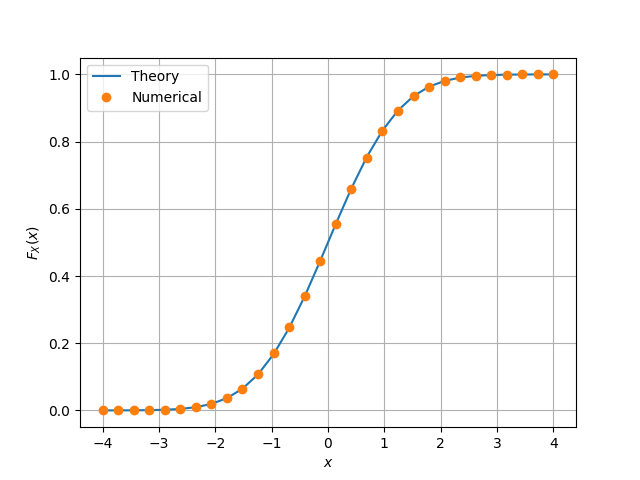
\includegraphics[width=\columnwidth]{gauss_cdf.png}
    \caption{The CDF of $X$}
    \label{fig:gauss_cdf}
\end{figure}
\textbf{properties of cdf}
\begin{itemize}
    \item $F_X(x)$ is a nondecreasing function of x for -$\infty < x < \infty$. 
    \item The CDF, $F_X(x)$ ranges from 0 to 1. This makes sense since $F_X(x)$ is a probability.
    \item If the maximum value of $X$ is b, \\then $F_X(b)$ = 1 \\
\end{itemize} 
$F_X(x) = P(X\le x) = \frac{1}{\sqrt{2\pi}}\int_{-\infty}^{\infty}e^{-\frac{x^2}{2}} dx$\\
The $Q$ function is defined as:
\begin{align}\label{q}
    Q(x) = 1 - F_X(x)
\end{align}
Hence,we can use eqn\eqref{q} to calculate $F_X(x)$\\


\item
Load gau.dat in python and plot the empirical PDF of $X$ using the samples in gau.dat. The PDF of $X$ is defined as
\begin{align}
p_{X}(x) = \frac{d}{dx}F_{X}(x)
\end{align}
What properties does the PDF have?

\solution The PDF of $X$ is plotted in Fig. \ref{fig:gauss_pdf}
using the code below 
\begin{lstlisting}
   $ wget https://github.com/jarpula-Bhanu/Random-numbers/blob/main/codes/pdf_plot.py
\end{lstlisting}
The above code is executed using command
\begin{lstlisting}
    $ wget python3 pdf_plot.py 
\end{lstlisting}
\begin{figure}[h]
    \centering
    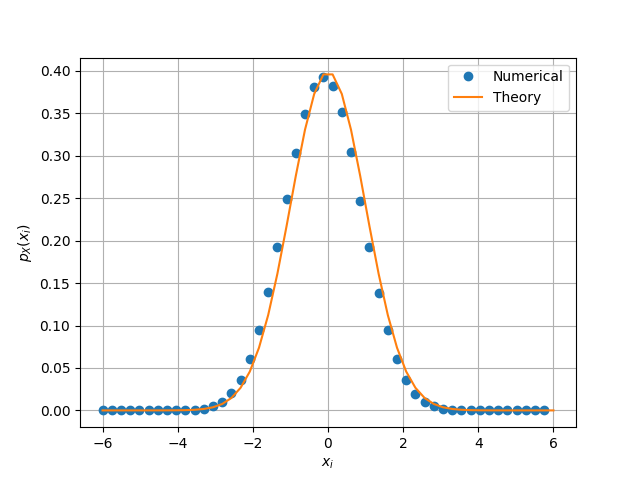
\includegraphics[width=\columnwidth]{gauss_pdf.png}
    \caption{The PDF of $X$}
    \label{fig:gauss_pdf}
\end{figure}

\textbf{properties of pdf}
\begin{itemize}
    \item PDF is symmetric about $X$ = 0 
    \item Graph is bell shaped
    \item Mean of graph is situated at the apex point of the bell.\\
\end{itemize}

\item Find the mean and variance of $X$ by writing a C program.

\solution
Download and run the following C code.

\noindent The C program can be downloaded using
\begin{lstlisting}
$ wget https://github.com/jarpula-Bhanu/Random-numbers/blob/main/codes/mean-var2-4.c
$ wget https://github.com/jarpula-Bhanu/Random-numbers/blob/main/codes/coeffs.h
\end{lstlisting}
Compile and execute the above C program using command
\begin{lstlisting}
$ gcc mean-var2-4.c -lm -o mean-var2-4.out
$ ./mean-var2-4.out
\end{lstlisting}

The mean of $X$ is 0.000326\\
The varience of $X$ is 1.000907\\

\item Given that 
\begin{align}
p_{X}(x) = \frac{1}{\sqrt{2\pi}}\exp\brak{-\frac{x^2}{2}}, -\infty < x < \infty,
\end{align}
repeat the above exercise theoretically.

\solution Verifying theoritically
    \begin{align}
        F_X(x) &= \int_{-\infty}^{x}\frac{1}{\sqrt{2\pi}}e^{-\frac{x^2}{2}}dx \\
        E[X]&= \frac{1}{\sqrt{2\pi}} \int_{-\infty}^{\infty}xe^{-\frac{x^2}{2}}dx 
    \end{align}
    Taking $\frac{x^2}{2} = t \rightarrow xdx = dt$
    \begin{align}
        E[X]&= \frac{1}{\sqrt{2\pi}} \int_{-\infty}^{\infty}e^{-t} dt = 0 \\
        E[X^2]&= \frac{1}{\sqrt{2\pi}} \int_{-\infty}^{\infty}x^2e^{-\frac{x^2}{2}}dx \\
        &= \frac{1}{\sqrt{2\pi}} \int_{-\infty}^{\infty}x(xe^{-\frac{x^2}{2}})dx \\
        &= \frac{1}{\sqrt{2\pi}} \bigg[-xe^{\frac{x^2}{2}}+\int_{-\infty}^{\infty}e^{-\frac{x^2}{2}} dx \bigg]_{-\infty}^{\infty} \\
        &= 1 \\
        \textbf{variance} &= E[X^2] - E[X]^2 = 1
    \end{align}
\end{enumerate}

\section{From Uniform to Other}
\begin{enumerate}[label=\thesection.\arabic*
,ref=\thesection.\theenumi]
\item
Generate samples of 
\begin{equation}
V = -2\ln\brak{1-U}
\end{equation}
and plot its CDF. 

\solution
Download the following files and execute the C program
\begin{lstlisting}
$ wget https://github.com/jarpula-Bhanu/Random-numbers/blob/main/codes/exrand.c
$ wget https://github.com/jarpula-Bhanu/Random-numbers/blob/main/codes/coeffs.h
\end{lstlisting}
Compile and execute the above C program using command
\begin{lstlisting}
$ gcc exrand.c -lm -o exrand.out
$ ./exrand.out
\end{lstlisting}
The above C program will save the values of V in log.dat\\

and the CDF is plotted in Figure \eqref{fig:V_cdf}.

\begin{lstlisting}
    $ wget https://github.com/jarpula-Bhanu/Random-numbers/blob/main/codes/cdf_plot3-1.py
\end{lstlisting}
The above code is executed using command
\begin{lstlisting}
    $ python3 cdf_plot3-1.py
\end{lstlisting}


\begin{figure}[h]
    \centering
    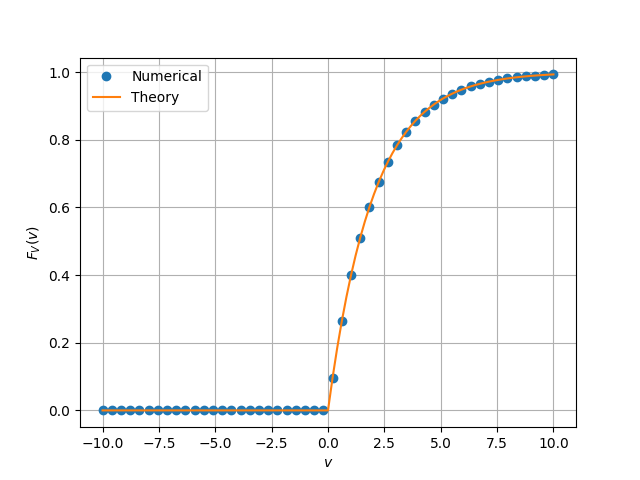
\includegraphics[width=\columnwidth]{V_cdf.png}
    \caption{The CDF of $V$}
    \label{fig:V_cdf}
\end{figure}

\item Find a theoretical expression for $F_V(x)$.\\
\solution
\begin{align}
    F_V(x) &= Pr(V \le x)\\
    &= Pr(-2 ln(1-U) \le x) \\
    &= Pr(U \le 1-e^{-\frac{x^2}{2}}) \\
    Pr(U<x) &= \int_0^x dx = x \\
    \therefore Pr(U \le 1-e^{-\frac{x^2}{2}}) &= 1-e^{-\frac{x^2}{2}} \\
    \rightarrow F_V(x) &=1-e^{-\frac{x^2}{2}}
\end{align}
%
\end{enumerate}

\section{Triangular Distribution}
\begin{enumerate}[label=\thesection.\arabic*
,ref=\thesection.\theenumi]
%
\item Generate 
	\begin{align}
		T = U_1+U_2
	\end{align}
    \solution
    Download the following files and execute the C program
    \begin{lstlisting}
    $ wget https://github.com/jarpula-Bhanu/Random-numbers/blob/main/codes/exrand.c
    $ wget https://github.com/jarpula-Bhanu/Random-numbers/blob/main/codes/coeffs.h
    \end{lstlisting}
    Compile and execute the above C program using command
    \begin{lstlisting}
    $ gcc exrand.c -lm -o exrand.out
    $ ./exrand.out
    \end{lstlisting}
The above code will generate T.dat file\\
\item Find the CDF of $T$.\\
\solution The CDF is plotted in Figure \eqref{fig:T_cdf}.

\begin{lstlisting}
    $ wget 
\end{lstlisting}
The above code is executed using command
\begin{lstlisting}
    $ python3 
\end{lstlisting}

\begin{figure}[h]
    \centering
    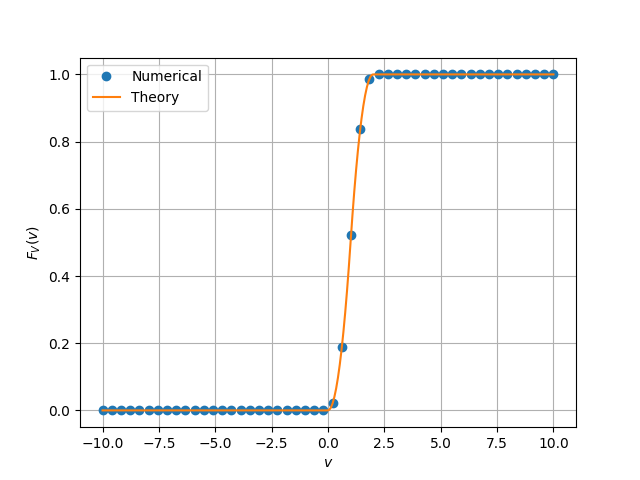
\includegraphics[width=\columnwidth]{T_cdf.png}
    \caption{The CDF of $T$}
    \label{fig:T_cdf}
\end{figure}
\item Find the PDF of $T$.\\
\solution The PDF is plotted in Figure \eqref{fig:T_Pdf}.

\begin{lstlisting}
    $ wget 
\end{lstlisting}
The above code is executed using command
\begin{lstlisting}
    $ python3 
\end{lstlisting}

\begin{figure}[h]
    \centering
    \includegraphics[width=\columnwidth]{T_Pdf.png}
    \caption{The PDF of $T$}
    \label{fig:T_Pdf}
\end{figure}
\item Find the theoretical expressions for the PDF and CDF of $T$.\\
\solution Let $T = U_1 + u_2$ where $U_1$ and $U_2$ are the uniform independent random varaible.We know ,pdf of $T$ is defined as 
\begin{align}
    f_T(t) &= \int_{-\infty}^{\infty}f_{U_1}(x)f_{U_2}(t-x)dx\\
    &=\int_{-\infty}^{\infty}f(x)f(t-x)dx
\end{align}
Since $U_1$ and $U_2$ are uniform random varaible between (0,1) they have the same density
i.e. $f_{U_1} = f_{U_2} = f$
\begin{align}
    f = \begin{cases}
        1 &= 0<x<1 \\
        0 & otherwise
    \end{cases}
\end{align}
The integrand $f(x)f(t-x)$ hence will have value either 0 or 1. \\
It is 1 when \\
$0<x<1$ and $0<t-x<1$ 
\begin{itemize}
    \item case 1:when $0<x<1$ , the limits run from $x=0$ to $x=t$ ,so
    \begin{align}
        f_T(t)=\int_0^t 1dx = t
    \end{align}
    \item case 2:when $1<x<2$ , the limits run from $x=t-1$ to $x=1$ ,so
    \begin{align}
        f_T(t)=\int_{t-1}^1 1dx = 2-t
    \end{align}
    \item case 3:when $x<0$ and $x>2$ ,The integrand is 0 so, 
    \begin{align}
        f_T(t)=0
    \end{align}
In terms of $T$ and $t$ we can Write
\begin{align}\label{pdf}
    \therefore f_T(t)=\begin{cases}
        t &0<t<1 \\
        2-t &1<t<2 \\
        0 &otherwise
    \end{cases}
\end{align}
\end{itemize}
Now the theoretical expression of cdf of $T$
\begin{align}
    F_T(t) &= \int_{0}^{t}f_T(t)dx\\
    &=\begin{cases}
        \int_{0}^{t} dt &0<t<1 \\
        \int_{0}^{t} (2-t)dt &1<t<2 \\
        \int_{0}^{2} (2-t)dt &t>2
    \end{cases} \\ \label{cdf}
    &=\begin{cases}
        0 & t<0 \\
        \frac{t^2}{2} &0<t<1\\
        2t - \frac{t^2}{2} & 1<t<2\\
        1 & t>2
    \end{cases}
\end{align}
\item Verify your results through a plot. \\
\solution The cdf i.e. eqn\ref{cdf} can be verified from Fig.\ref{fig:T_cdf}\\
and The pdf i.e. eqn\ref{pdf} can be verified from Fig.\ref{fig:T_Pdf}

\end{enumerate}

\section{Maximul Likelihood}
\begin{enumerate}[label=\thesection.\arabic*
,ref=\thesection.\theenumi]
\item Generate 
\begin{equation}
Y = AX+N,
\end{equation}
		where $A = 5 \text{ dB}, X \i \cbrak{1,-1}$,  is Bernoulli and $N \sim \gauss{0}{1}$.\\
\solution
\item Plot $Y$.\\
\solution
\item Guess how to estimate $X$ from $Y$.\\
\solution
\item
\label{ml-ch4_sim}
Find 
\begin{equation}
	P_{e|0} = \pr{\hat{X} = -1|X=1}
\end{equation}
and 
\begin{equation}
	P_{e|1} = \pr{\hat{X} = 1|X=-1}
\end{equation}
%
\solution
\item Find $P_e$.\\
%
\solution
\item
Verify by plotting  the theoretical $P_e$.\\  
\solution
		\end{enumerate}

\section{Gaussian to Other}
\begin{enumerate}[label=\thesection.\arabic*
,ref=\thesection.\theenumi]
\item
Let $X_1 \sim  \gauss{0}{1}$ and $X_2 \sim  \gauss{0}{1}$. Plot the CDF and PDF of
%
\begin{equation}
V = X_1^2 + X_2^2
\end{equation}
\solution The following codes plots\\
 Fig.\ref{fig:6.1_cdf} - CDF of $V$ and Fig.\ref{fig:6.1_pdf} - PDF of $V$
\begin{lstlisting}
    $ wget 
    $ wget 
\end{lstlisting}
run above python code using the command
\begin{lstlisting}
    $ python3 
    $ python3 
\end{lstlisting}
\begin{figure}[h]
    \centering
    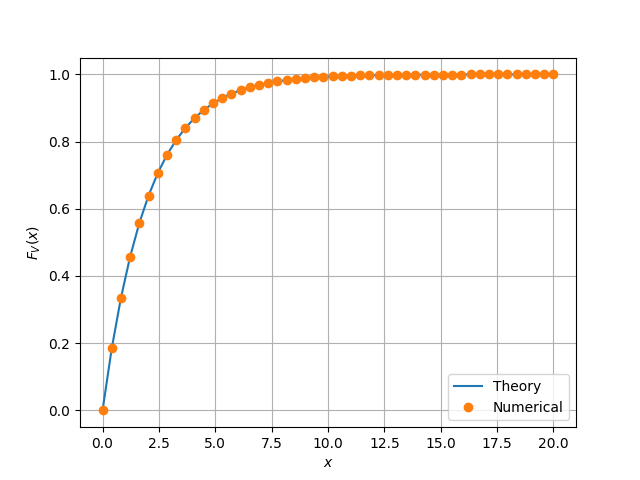
\includegraphics[width=\columnwidth]{6.1_cdf.png}
    \caption{The CDF of $V$}
    \label{fig:6.1_cdf}
\end{figure}
\begin{figure}[h]
    \centering
    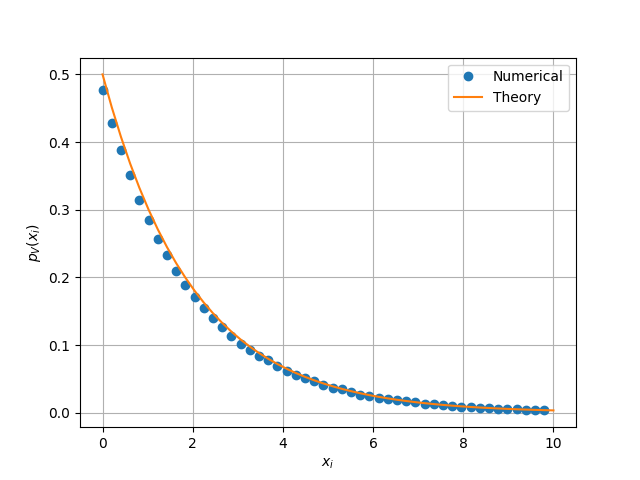
\includegraphics[width=\columnwidth]{6.1_pdf.png}
    \caption{The PDF of $V$}
    \label{fig:6.1_pdf}
\end{figure}
%
%
%
\item
If
%
\begin{equation}
F_{V}(x) = 
\begin{cases}
1 - e^{-\alpha x} & x \geq 0 \\
0 & x < 0,
\end{cases}
\end{equation}
%
find $\alpha$.\\
\solution For the value $\alpha$ = 0.5, the theory matches the stimulation\\
The following code plots the Fig.\ref{fig:6.2_cdf}
\begin{lstlisting}
    $ wget
\end{lstlisting}
run above python code using the command
\begin{lstlisting}
    $ python3
\end{lstlisting}
\begin{figure}[h]
    \centering
    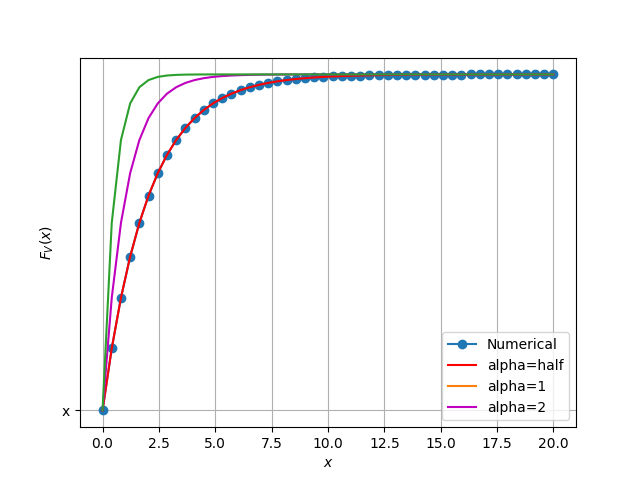
\includegraphics[width=\columnwidth]{6.2_cdf.png}
    \caption{The CDF of $V$}
    \label{fig:6.2_cdf}
\end{figure}

%
\item
\label{ch3_raleigh_sim}
Plot the CDF and PDf of
%
\begin{equation}
A = \sqrt{V}
\end{equation}
%
\solution The following codes plots\\
 Fig.\ref{fig:6.3_cdf} - CDF of $A$ and Fig.\ref{fig:6.3_pdf} - PDF of $A$
\begin{lstlisting}
    $ wget 
    $ wget 
\end{lstlisting}
run above python code using the command
\begin{lstlisting}
    $ python3 
    $ python3 
\end{lstlisting}
\begin{figure}[h]
    \centering
    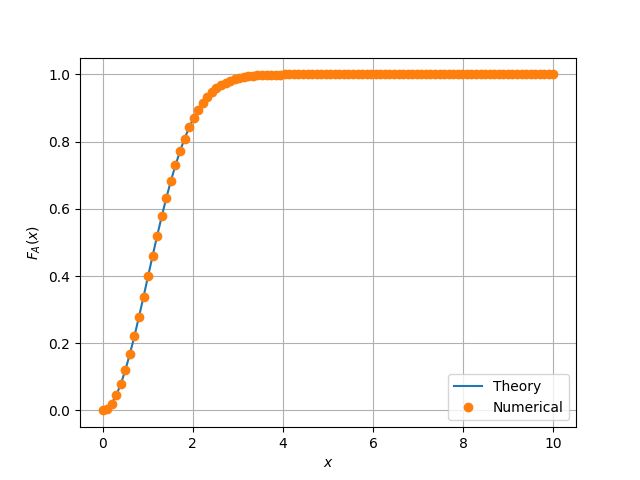
\includegraphics[width=\columnwidth]{6.3_cdf.png}
    \caption{The CDF of $A$}
    \label{fig:6.3_cdf}
\end{figure}
\begin{figure}[h]
    \centering
    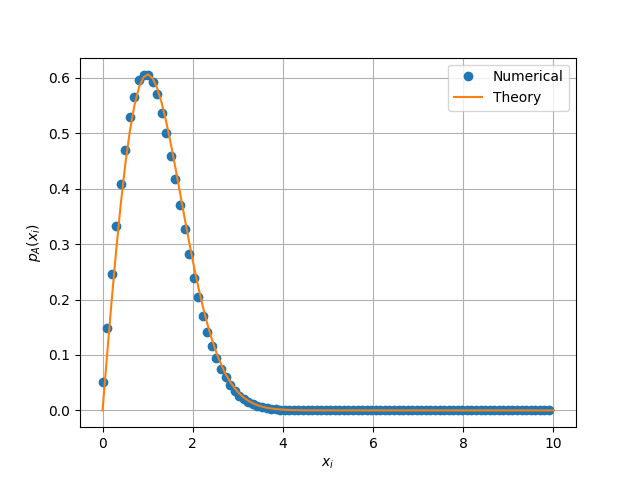
\includegraphics[width=\columnwidth]{6.3_pdf.png}
    \caption{The PDF of $A$}
    \label{fig:6.3_pdf}
\end{figure}


\end{enumerate}


\section{Conditional Probability}
\begin{enumerate}[label=\thesection.\arabic*
,ref=\thesection.\theenumi]
\item
\label{ch4_sim}
Plot 
\begin{equation}
P_e = \pr{\hat{X} = -1|X=1}
\end{equation}
%
for 
\begin{equation}
Y = AX+N,
\end{equation}
where $A$ is Raleigh with $E\sbrak{A^2} = \gamma, N \sim \gauss{0}{1}, X \in \brak{-1,1}$ for $0 \le \gamma \le 10$ dB.\\
%
\solution see Fig. \ref{fig:7.4-gamma}\\
\item
Assuming that $N$ is a constant, find an expression for $P_e$.  Call this $P_e(N)$\\
%
\solution   The estimathed value $\hat{X}$ is given by 
\begin{align}
    \hat{X} &=
    \begin{cases}
        1  &Y>0
        \\
        -1 &Y<0
    \end{cases}
\end{align}
For $X$ = 1
\begin{align}
    Y &= A + N \\
    P_e &= \pr{\hat{X} = -1|X=1}\\
    &=\pr{Y<0|X=1} \\
    &=\pr{A < -N} \\
    &= F_A(-N)\\
    &= \int_{-\infty}^{-N}f_A(x)dx
\end{align}
By definition 
\begin{align}
    f_A(x) &=
    \begin{cases}
        \frac{x}{\sigma^2} exp(-\frac{x^2}{2\sigma^2}) & x\ge 0
        \\
        0 & otherwise
    \end{cases}
\end{align}
If $N > 0, f_A(x) = 0$. then 
\begin{align}
    P_e = 0
\end{align}
if $N < 0$, then 
\begin{align}
    P_e(N) &= \int_{-\infty}^{-N}f_A(x)dx \\
    &= \int_{-\infty}^{0}0dx + \int_{0}^{-N}f_A(x)dx\\
    &= \int_{0}^{-N}\frac{x}{\sigma^2} exp(-\frac{x^2}{2\sigma^2}) dx\\
    &=1 - exp(-\frac{N^2}{2\sigma^2})
\end{align}

\begin{align}\label{2}
\therefore   P_e(N) &=
    \begin{cases}
        1 - exp(-\frac{N^2}{2\sigma^2}) & N<0
        \\
        0 & otherwise 
    \end{cases}
\end{align}
\item
%
\label{ch4_anal}
For a function $g$,
\begin{equation}
E\sbrak{g(X)} = \int_{-\infty}^{\infty}g(x)p_{X}(x)\, dx
\end{equation}
%
Find $P_e = E\sbrak{P_e(N)}$.\\
%
\solution since $N \sim \gauss{0}{1}$,
\begin{align}
    P_N(x) = \frac{1}{\sqrt{2\pi}} exp(-\frac{x^2}{2})
\end{align}
and form eqn\ref{2} 
\begin{align}
    P_e(N) &=
        \begin{cases}
            1 - exp(-\frac{N^2}{2\sigma^2}) & N<0
            \\
            0 & otherwise 
        \end{cases}\\
        P_e(N) &= E[P_e(N)]=\int_{-\infty}^(\infty)P_e(x)P_N(x)dx
    \end{align} 
If $x<0 , P_e(x) = 0$ and using the fact that for an even function
\begin{align}
    \int_{-\infty}^{\infty} f(x) = 2\int_{-\infty}^{0} f(x)
\end{align}

we get 
\begin{align}
    P_e &= \frac{1}{\sqrt{2\pi}} \int_{-\infty}^{0} exp\bigg({-\frac{x^2}{2}}\bigg)\bigg(1-exp\bigg({-\frac{x^2}{2\sigma^2}}\bigg)\bigg)dx\\
    &= \frac{1}{2\sqrt{2\pi}}\int_{-\infty}^{\infty} exp\bigg({-\frac{x^2}{2}}\bigg)dx\\ &- \frac{1}{2\sqrt{2\pi}}\int_{-\infty}^{\infty} exp\bigg({-\frac{(1+\sigma^2)x^2}{2\sigma^2}}\bigg)dx\\
    &= \frac{\sqrt{2\pi - \sqrt{\frac{\pi(2\sigma^2)}{1+\sigma^2}}}}{2\sqrt{2\pi}}\\
    &=\frac{1}{2} - \frac{1}{2}\sqrt{\frac{\sigma^2}{1+\sigma^2}}\\    
\end{align}
For a Rayleigh Distribution with scale = $\sigma$,
\begin{align}
    E[A^2] &= 2\sigma^2 \\
    \gamma &= 2\sigma^2 \\
    \therefore P_e &=\frac{1}{2} - \frac{1}{2}\sqrt{\frac{\gamma}{2+\gamma}}
\end{align}

\item
Plot $P_e$ in problems \ref{ch4_sim} and \ref{ch4_anal} on the same graph w.r.t $\gamma$.  Comment.\\
\solution  The following code plots Fig. \ref{fig:7.4-gamma}\\
$P_e$ is plotted w.r.t $\gamma$
\begin{lstlisting}
$ wget
\end{lstlisting}
The above code is executed using command
\begin{lstlisting}
$ python3 
\end{lstlisting}
\begin{figure}[h]
    \centering
    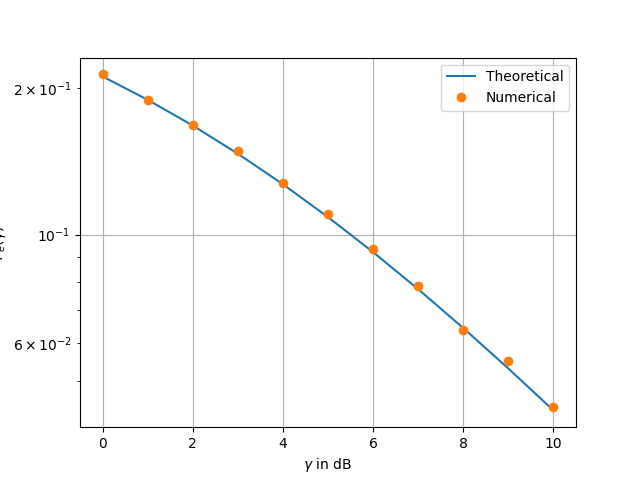
\includegraphics[width=\columnwidth]{7.4-gamma.png}
    \caption{$P_e$ w.r.t $\gamma$}
    \label{fig:7.4-gamma}
\end{figure}


\end{enumerate}


\section{Two Dimensions}
Let 
\begin{equation}
\mbf{y} = A\mbf{x} + \mbf{n},
\end{equation}
where 
\begin{align}
x &\in \brak{\mbf{s}_0,\mbf{s}_1}, 
\mbf{s}_0 = 
\begin{pmatrix}
1 
\\
0
\end{pmatrix},
\mbf{s}_1 = 
\begin{pmatrix}
0 
\\
1
\end{pmatrix}
\\
\mbf{n} &= 
\begin{pmatrix}
n_1
\\
n_2
\end{pmatrix},
n_1,n_2 \sim \gauss{0}{1}.
\end{align}
%
\begin{enumerate}[label=\thesection.\arabic*
,ref=\thesection.\theenumi]
%%
\item
\label{ch5_fsk}
Plot 
%
\begin{equation}
\mbf{y}|\mbf{s}_0 \text{ and } \mbf{y}|\mbf{s}_1
\end{equation}
%
on the same graph using a scatter plot.\\
%
\solution The following code plots the scatter plot when 
$\textbf{x} = \textbf{s}_0$ and $\textbf{x} = \textbf{s}_1$ in Fig.\ref{fig:8.1_scatter}
\begin{lstlisting}
    $ wget
    \end{lstlisting}
    The above code is executed using command
    \begin{lstlisting}
    $ python3 
    \end{lstlisting}
    \begin{figure}[h]
        \centering
        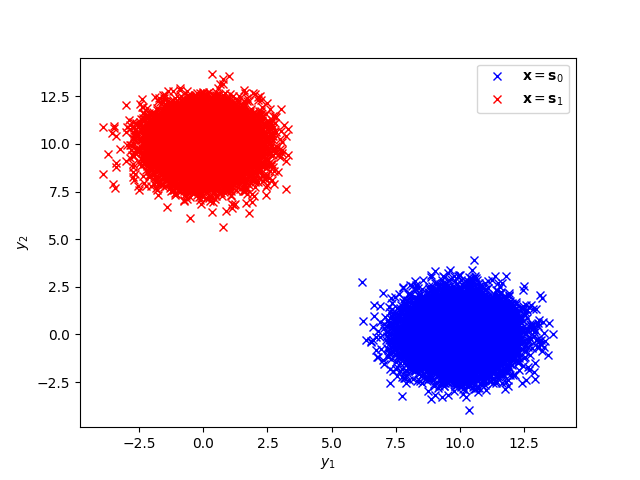
\includegraphics[width=\columnwidth]{8.1_scatter.png}
        \caption{Scatter plot of $Y$ for $A$ = 10}
        \label{fig:8.1_scatter}
    \end{figure}
\item
For the above problem, find a decision rule for detecting the symbols $\mbf{s}_0 $ and $\mbf{s}_1$.\\
%
\solution The multivariate Gaussian distribution is defined as
%
\begin{multline}
\label{eq:multivariate}
p_{\mathbf{x}}(x_1,\dots,x_k)
\\
=\frac{1}{\sqrt{\brak{2\pi}^k\abs{\mbf{\Sigma}}}}\exp\cbrak{-\frac{1}{2}\brak{\mathbf{x}-\mbf{\mu}}^T\mbf{\Sigma}^{-1}\brak{\mathbf{x}-\mbf{\mu}}}
\end{multline}
%
where $\mbf{\mu}$ is the mean vector, $\mbf{\Sigma} = E\sbrak{\brak{\mathbf{x}-\mbf{\mu}}\brak{\mathbf{x}-\mbf{\mu}}^T}$ is the covariance matrix and $\abs{\mbf{\Sigma}}$ is the determinant of $\mbf{\Sigma}$.
For a bivariate gaussian distribution,
{\small
\begin{multline}
\label{eq:bivariate}
p(x,y)= \frac{1}{2\pi \sigma_x\sigma_y\sqrt{1-\rho^2}}\exp\lsbrak{-\frac{1}{2\brak{1-\rho^2}}}
\\
\times \rsbrak{\cbrak{\frac{\brak{x-\mu_x}^2}{\sigma_x^2}+\frac{\brak{y-\mu_y}^2}{\sigma_y^2}-\frac{2\rho\brak{x-\mu_x}\brak{y-\mu_y}}{\sigma_x\sigma_y}}}
\end{multline}
}
%
where
%
\begin{align}
%\mbf{\mu}=
&\mbf{\mu}=
\begin{pmatrix*}
\mu_x \\
\mu_y
\end{pmatrix*},
\mbf{\Sigma} = 
\begin{pmatrix*}%[r]
\sigma_x^2 & \rho\sigma_x\sigma_y \\
\rho\sigma_x\sigma_y & \sigma_y^2
\end{pmatrix*},\\
&\rho = \frac{E\sbrak{\brak{x - \mu_x}\brak{y-\mu_y}}}{\sigma_x\sigma_y}.
\end{align}
%
\begin{align}
    \mbf{y}|s_0 &= 
    \begin{pmatrix}
    A+n_1 \\
    n_2
    \end{pmatrix}\\
    \mbf{y}|s_1 &=  
    \begin{pmatrix}
    n_1 \\
    A+n_2
    \end{pmatrix}
    \end{align}
    Substituting these values in (\ref{eq:bivariate}),
    \begin{multline}
    \label{gauss_mutl_var1}
    p\brak{\mbf{y}|s_0} = \frac{1}{2\pi\sigma_{y_1}\sigma_{y_2}\sqrt{1-\rho_1^2}}\exp\lsbrak{-\frac{1}{2\brak{1-\rho_1^2}}}
    \\
    \times \rsbrak{\cbrak{\frac{\brak{y_1-A}^2}{\sigma_{y_1}^2}+\frac{\brak{y_2}^2}{\sigma_{y_2}^2}-\frac{2\rho_1\brak{y_1-A}\brak{y_2}}{\sigma_{y_1}\sigma_{y_2}}}}
    \end{multline}
    \begin{multline}
    \label{gauss_mutl_var2}
    p\brak{\mbf{y}|s_1} = \frac{1}{2\pi\sigma_{y_1}\sigma_{y_2}\sqrt{1-\rho_2^2}}\exp\lsbrak{-\frac{1}{2\brak{1-\rho_2^2}}}
    \\
    \times \rsbrak{\cbrak{\frac{\brak{y_1}^2}{\sigma_{y_1}^2}+\frac{\brak{y_2-A}^2}{\sigma_{y_2}^2}-\frac{2\rho_2\brak{y_1}\brak{y_2-A}}{\sigma_{y_1}\sigma_{y_2}}}}
    \end{multline}
    where,
    \begin{align}
    \label{rho_sig_val}
    \rho_1 = E[(y_1-A)(y_2)] &= E[n_1 n_2] = 0, \nonumber \\
    \rho_2 = E[(y_1)(y_2-A)] &= E[n_1 n_2] = 0, \nonumber \\
    \sigma_{y_1} = \sigma_{y_2} &= 1
    \end{align}
    For equiprobably symbols, the MAP criterion is defined as
    %
    \begin{align}
    \label{eq:map_bfsk_dec}
    p\brak{\vec{y}|s_0} &\dec{s_0}{s_1} p\brak{\vec{y}|s_1}
    \end{align}
    Using (\ref{gauss_mutl_var1}) and (\ref{gauss_mutl_var2}) and substituting the values from (\ref{rho_sig_val}),  we get
    \begin{align}
    (y_1 -A)^2 + y_2^2 \dec{s_1}{s_0} y_1^2 + (y_2 - A)^2
    \end{align}
    On simplifying, we get the decision rule is
    \begin{align}
    \label{eq:decision_rule}
    y_1 \dec{s_0}{s_1} y_2
    \end{align}

\item
Plot 
\begin{equation} 
P_e = \pr{\hat{\mbf{x}} = \mbf{s}_1|\mbf{x} = \mbf{s}_0}
\end{equation}
with respect to the SNR from 0 to 10 dB.\\
%
\solution The following code plots Fig. \ref{fig:8.3_snr}\\
\begin{lstlisting}
$ wget
\end{lstlisting}
The above code is executed using command
\begin{lstlisting}
$ python3 
\end{lstlisting}
\begin{figure}[h]
    \centering
    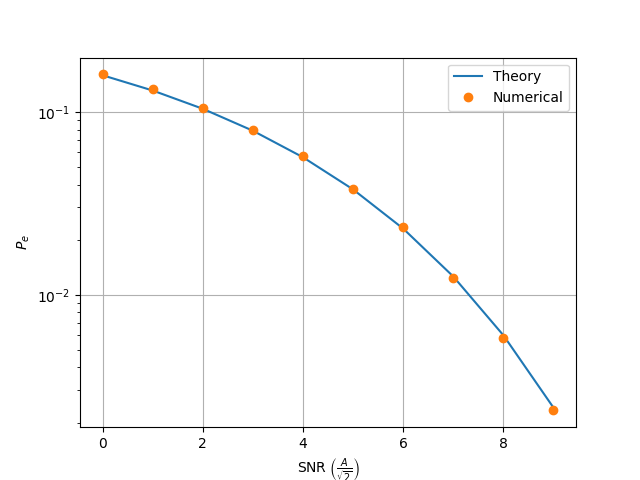
\includegraphics[width=\columnwidth]{8.3_snr.png}
    \caption{$P_e$ w.r.t SNR from 0 to 10 dB}
    \label{fig:8.3_snr}
\end{figure}
\item
Obtain an expression for $P_e$. Verify this by comparing the theory and simulation plots on the same graph.\\
%
\solution 
\begin{align}
P_e = \pr{\hat{\mbf{x}} = \mbf{s}_1|\mbf{x} = \mbf{s}_0}
\end{align}
Given that $\mbf{s}_0$ was transmitted, the received signal is
\begin{align}
\mbf{y}|\mbf{s}_0 = \begin{pmatrix} A \\ 0 \end{pmatrix} + \begin{pmatrix} n_1 \\ n_2 \end{pmatrix}
\end{align}
From (\ref{eq:decision_rule}), the probability of error is given by 
\begin{align}
P_e &= \pr{y_1 < y_2 |\mbf{s}_0} = \pr{A+n_1 < n_2}\\
&= \pr{n_2 - n_1 > A}
\end{align}
Note that $n_2 - n_1 \sim \gauss{0}{2}$. Thus,
\begin{align}
P_e &= \pr{\sqrt{2}w > A}\\
\pr{w > \dfrac{A}{\sqrt{2}}}\\
\Rightarrow P_e &= \qfunc{\frac{A}{\sqrt{2}}}
\end{align}


\end{enumerate}

\end{document}